\documentclass[12pt,a4paper]{article}

\usepackage[utf8]{inputenc}
\usepackage[ngerman]{babel}
\usepackage[T1]{fontenc}
\usepackage{amsmath}
\usepackage{amsfonts}
\usepackage{amssymb}
\usepackage{graphicx}
\usepackage[left=2cm,right=2cm,top=2cm,bottom=2cm]{geometry}
\usepackage{multicol}
\usepackage{booktabs}
\usepackage[hidelinks]{hyperref}
\usepackage{tikz}
\usepackage{pgfplots}
\usepackage{blindtext}
\usepackage{array}
\usepackage{multirow}
\usepackage{bigdelim}
\usepackage{colortbl}
\usepackage{fancyhdr} 
\usepackage{tabularx}
\usepackage{xcolor}
\usepackage{color}
\usetikzlibrary{decorations.text}
\usetikzlibrary{tikzmark}
\pagestyle{fancy} 
	\fancyhf{} 
	\fancyhead[L]{
\includegraphics[scale=0.05]{Bilder/dhbw.png}} 
	\fancyhead[C]{\slshape Projektmanagement} 
	\fancyhead[R]{\slshape LaTeX Version}

\usepackage{helvet}
\renewcommand{\familydefault}{\sfdefault}

\author{\slshape Robin Rausch, Florian Maslowski, Ozan Akzebe}
\title{Projektmanagement}
\date{\slshape \today}
\begin{document}
\maketitle
\section{Fragenkatalog}
\begin{enumerate}
	\item Wie ist ein Projekt definiert (Eigenschaften)?
		\begin{enumerate}
		\item[] Einmaligkeit der Bedingungen 
		\item[] Zielvorgabe 
		\item[] Begrenzungen von Ressourcen (Zeit, Finanzen, Personal)
		\item[] Abgrenzung zu anderen Vorhaben 
		\item[] Projektspezifische Organisation 
		\end{enumerate}
	\item Was ist Projektmanagement?
		\begin{enumerate}
		\item[] Führungskonzept zur zielorientierten Durchführung großer Vorhaben 
		\item[] Gesamtheit der Führungsaufgaben 
			\begin{enumerate}
			\item[*] Zielsetzung
			\item[*] Planung
			\item[*] Steuerung
			\item[*] Überwachung
			\end{enumerate}
		\item[] Führungsaufbaus (Projektorganisation)
		\item[] Führungstechnik (Führungsstil) 
		\item[] Führungsmittel (Methoden) 
		\end{enumerate}
	\item Warum gehen Projekte schief?
		\begin{enumerate}
		\item[] Unklare Definition der Projektziele und Aufgaben 
		\item[] Falsche Einschätzung von Risiken 
		\item[] Verschiedene Projektvorstellungen die nicht abgestimmt werden  
		\item[] Ungenügende Kommunikation im Team 
		\end{enumerate}
	\item Was ist die Aufgabe eines Projektmanagers?
		\begin{enumerate}
		\item[] Aufgabenverteilung und Priorisierung 
		\item[] Kommunikation zwischen Gruppen 
		\item[] Ziele festlegen und erreichen  
		\item[] Konfliktbewältigung 
		\item[] Sicherstellung der Wirtschaftlichkeit  
		\item[] Entscheidung über Inhalt und Projektablauf 
		\end{enumerate}
	\item Welches sind die drei Säulen der PRM-Kompetenz?
		\begin{enumerate}
		\item[] Fachliche Kompetenz 
		\item[] Soziale Kompetenz
		\item[] Wirtschaftliche Kompetenz 
		\end{enumerate}
	\item Wozu dient das PM-BoK (Body of Knowledge)?
		\begin{enumerate}
		\item[] Kann Firmenspezifisch angewendet werden 
		\item[] Informationen über die Wissensgebiete im Projektmanagement  
			\begin{enumerate}
			\item[*] Integrationsmanagement
			\item[*] Umfangsmanagement
			\item[*] Terminmanagement
			\item[*] Kostenmanagement
			\item[*] Qualitätsmanagement
			\item[*] Personalmanagement
			\item[*] Kommunikationsmanagement
			\item[*] Risikomanagement
			\item[*] Beschaffungsmanagement
			\end{enumerate}
		\end{enumerate}
	\item Wozu benötigt man Ziele im Projekt und wie unterteilt man diese?
		\begin{enumerate}
		\item[] Um den Soll-Zustand festzustellen (Was soll erreicht werden?) 
		\item[] Unterteilung in: 
			\begin{enumerate}
			\item[*] Funktionale Ziele (Qualitative Ziele)
			\item[*] Operationale Ziele (Quantitative Ziele)
			\end{enumerate}
		\end{enumerate}
	\item An welches Prinzip sollten sich Ziele anlehnen?
		\begin{enumerate}
		\item[] SMART: 
			\begin{enumerate}
			\item[*] S: Spezifisch
			\item[*] M: Messbar
			\item[*] A: Angemessen
			\item[*] R: Realistisch
			\item[*] T: Terminierbar
			\end{enumerate}
		\end{enumerate}
	\item Welche Ziele dienen zur Messung des Erfolgs eines Projekts?
		\begin{enumerate}
		\item[] Sachziele
		\item[] Terminziele
		\item[] Kostenziele
		\end{enumerate}
	\item Was versteht man unter dem magischen Dreieck im PRM?
		\begin{enumerate}
		\item[] Zirkuläre Abhängigkeiten
		\item[] \includegraphics[scale=0.3]{Bilder/magischesDreieck.PNG}
		\end{enumerate}
	\item Was ist ein Zielsystem?
		\begin{enumerate}
		\item[] Ein Oberziel wird in mehrere Ziele unterteilt
		\end{enumerate}
	\item Verschiedene Projektorganisationen
	\begin{enumerate}
		\item[] Einfluß Projektmanagement
		\item[] 
		\item[] Matrix Projektmanagement
		\item[] 
		\item[] Reines Projektmanagement
		\begin{enumerate}
			\item[] 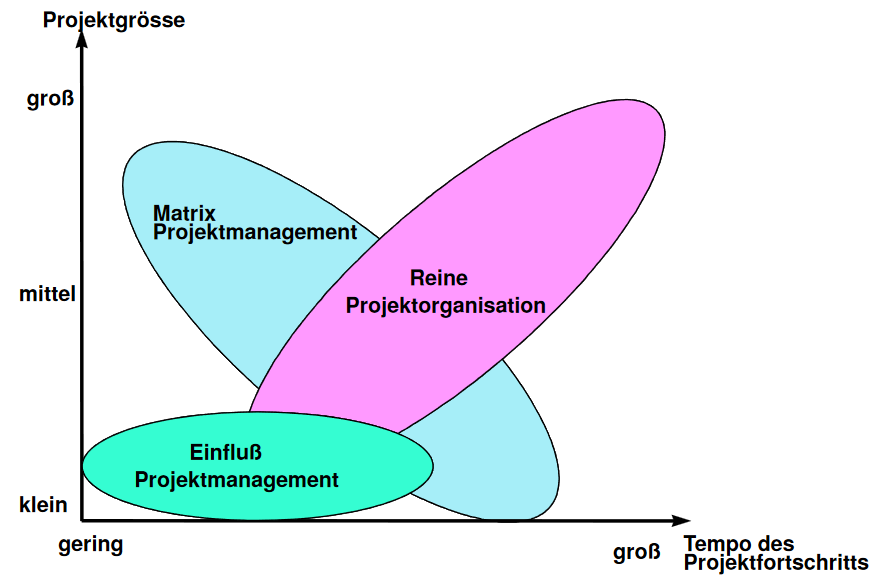
\includegraphics[scale=0.6]{Bilder/projektorganisationenWirksamkeit.PNG}
		\end{enumerate}
	\end{enumerate}
	\item Warum gibt es in der Analysephase eine solch große Begriffsvielfalt an Dokumenten?
	\begin{enumerate}
		\item Es gibt keine internationale Normung und somit viele verschiedene Begriffe und vorallem auch viele Synonyme.
	\end{enumerate}
	\item Was unterscheidet in der Projektphase das Lasten- vom Pflichtenheft?
	\begin{enumerate}
		\item Das Lastenheft wird zuerst erstellt und beeinhaltet nur die Forderungen des Auftraggebers, während das Pflichtenheft auf dem Lastenheft aufbaut und deutlich spezifischer ist. Das Pflichtenheft dient als Vertrags- und Einigungsgrundlage.
	\end{enumerate}
	\item Was beschreibt das Lastenheft und wer erstellt es?
	\begin{enumerate}
		\item Das Lastenheft beschreibt die Anforderungen an das Projekt und wird vom Auftraggeber erstellt.
	\end{enumerate}
	\item Was beschreibt das Pflichtenheft und wer erstellt es?
	\begin{enumerate}
		\item Das Pflichtenheft beinhaltet die detallierte Umsetzung des Projektes und wird vom Auftragnehmer(Projektleiter) erstellt.
	\end{enumerate}
	\item Wozu dient der Projektplan(Projektakte) und was enthält er?
	\begin{enumerate}
		\item Kostenplan
		\item Zeitplan
		\item Risikoplan
		\item ...
	\end{enumerate}
	\item Was versteht man unter einem Projekttagebuch und was enthält es?
	\begin{enumerate}
		\item Ablauf und Übersicht vom Projekt und dient zur Übersicht
	\end{enumerate}
	\item Was ist ein Projektstrukturplan und wozu wird er verwendet?
	\begin{enumerate}
		\item Darstellung der Teilprojekte und ? 
		\item Dient zur Übersicht
	\end{enumerate}
	\item Warum und wie strukturieren wir Projekte?
	\begin{enumerate}
		\item Zusammenhänge aufdecken und verstehen
		\item Übersichtlichkeit mithilfe von Baumstruktur
	\end{enumerate}
	\item Nach welchem Vorgehen werden Projekte strukturiert und wie entscheide ich mich für eine Methode?
	\begin{enumerate}
		\item Top-Down oder Bottom-Up
		\item Entscheidung abhängig davon, wie viel Erfahrung vorhanden ist und ob die Ziele klar definiert sind
	\end{enumerate}
	\item Wie detalliert strukturieren wir Projekte?
	\begin{enumerate}
		\item So detalliert wie notwendig.
		\item Bis zu einer bestimmten zeitlichen Ebene
	\end{enumerate}
	\item Wie sind AP's definiert und auf welcher Ebene des PSP's sind diese zu finden?
	\begin{enumerate}
		\item Unterste Ebene des PSP's
		\item Beinhalten Kostenschätzung, Zeitschätzung, \dots
		\item Hat Verantwortlichkeiten
	\end{enumerate}
	\item Was ist beim Schätzen von Aufwendungen wichtig?
	\begin{enumerate}
		\item Je mehr Wissen und Erfahrung, desto besser bzw. genauer wird die Schätzung
	\end{enumerate}
	\item Welche Schätzmethoden kennen sie und erklären sie diese?
	\begin{enumerate}
		\item Planning Poker
		\begin{enumerate}
			\item Team schätzt unabhängig von einander eine Task
			\item Wahl zwischen verschieden Fibonacci-Zahlen
			\item Team muss einstimmig wählen
			\item Bei unterschiedlichen Schätzungen wird sich drüber unterhalten und erneut geschätzt
		\end{enumerate}
		\item Dreipunkt-Methode
		\begin{enumerate}
			\item optimistische Schätzung
			\item mittlere Schätzung
			\item pessimistische Schätzung
		\end{enumerate}
	\end{enumerate}
	\item Wann ist ein Projekt wirtschaftlich?
	\begin{enumerate}
		\item Wenn der Gewinn höher ist als die Kosten
	\end{enumerate}
	\item Frage
	\begin{enumerate}
		\item Antwort
	\end{enumerate}
	\item Frage
	\begin{enumerate}
		\item Antwort
	\end{enumerate}
	\item Frage
	\begin{enumerate}
		\item Antwort
	\end{enumerate}
	\item Frage
	\begin{enumerate}
		\item Antwort
	\end{enumerate}
	\item Frage
	\begin{enumerate}
		\item Antwort
	\end{enumerate}
	\item Frage
	\begin{enumerate}
		\item Antwort
	\end{enumerate}
	\item Frage
	\begin{enumerate}
		\item Antwort
	\end{enumerate}
\end{enumerate}
\end{document}